\section{Vorsteuerung}
Die Simulationen zeigen, dass eine Vorsteuerung mit der Standardauslegung
(Inversion vom Prozess) ohne eine Anpassung des Reglers einen negativen
Einfluss hat.

\begin{figure}[h!]
    \centering
    \begin{subfigure}{0.475\textwidth}
        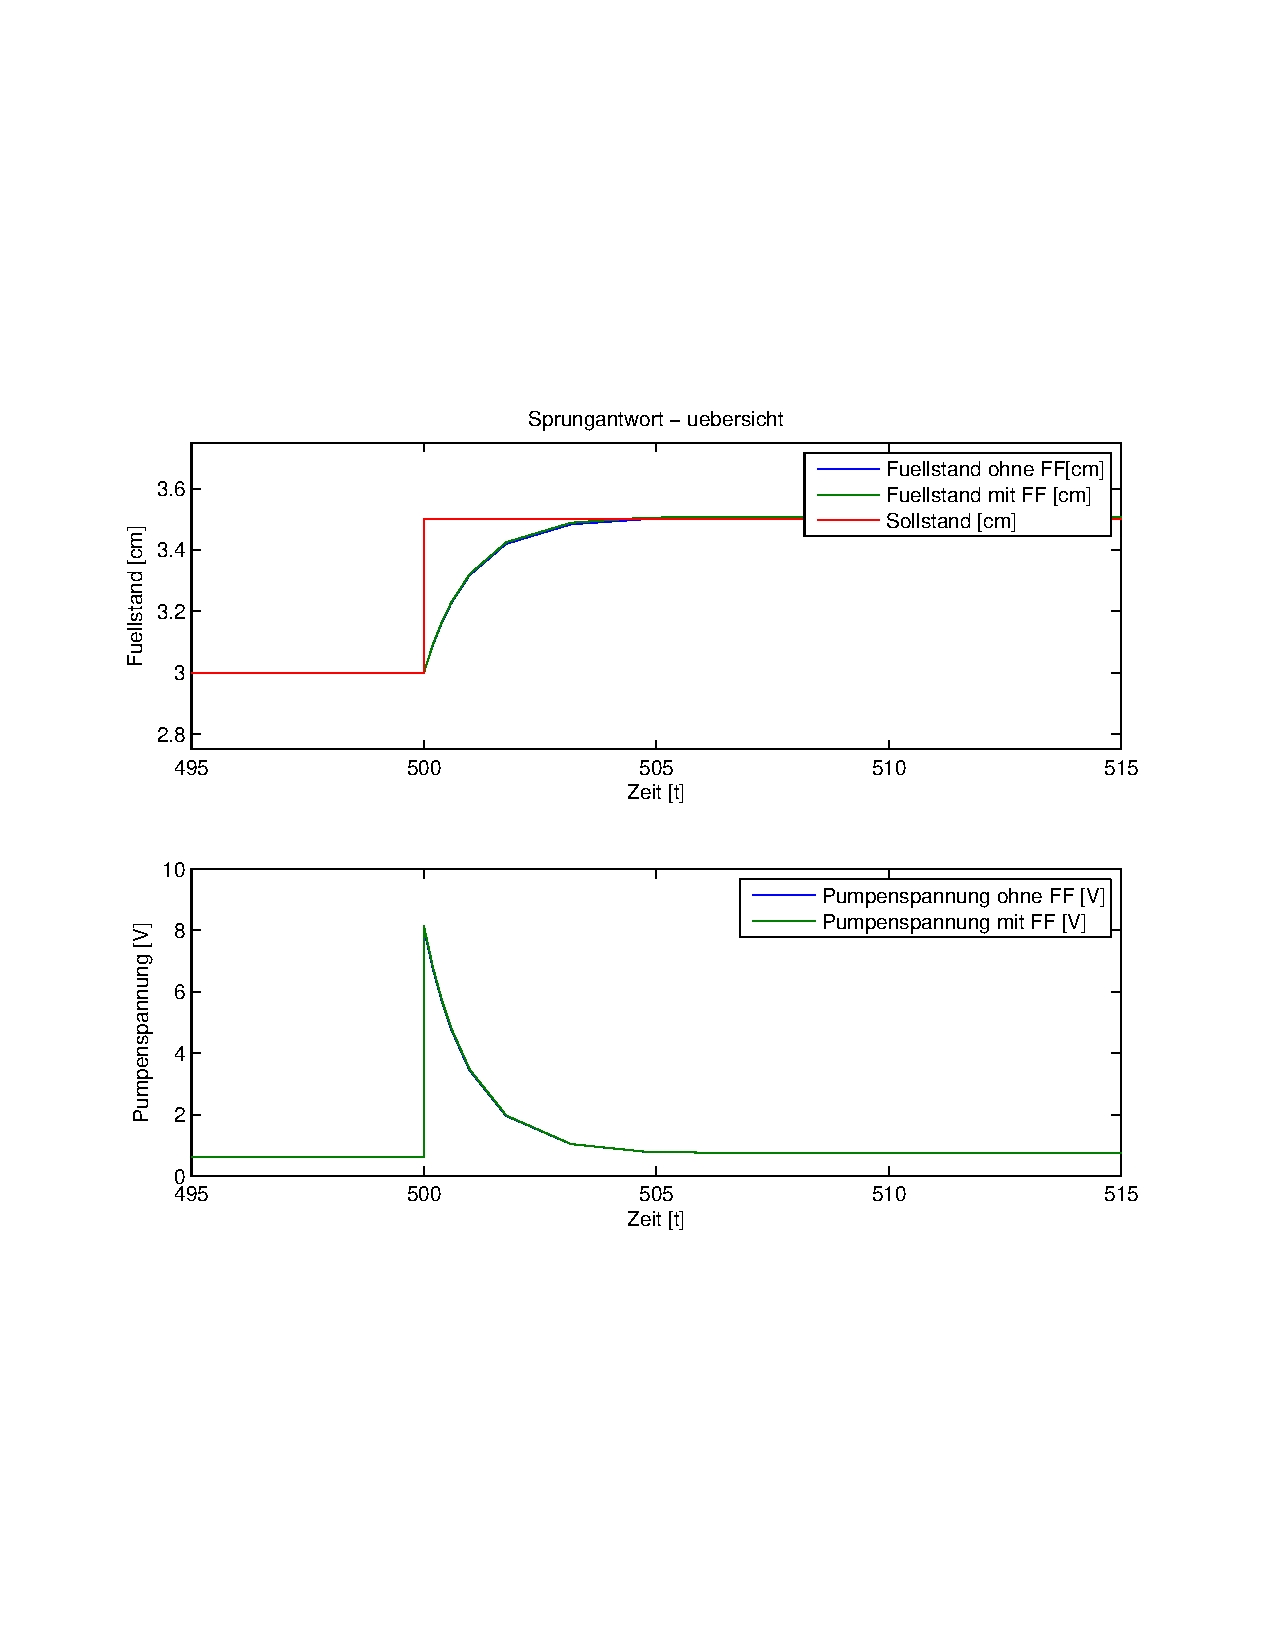
\includegraphics[width=1.\textwidth]{13/L5_step_overview_plot.pdf}
        \caption{Schrittantwort im Arbeitsbereich von $G_5(s)$}
    \end{subfigure}
    \hfill{}
    \begin{subfigure}{0.475\textwidth}
        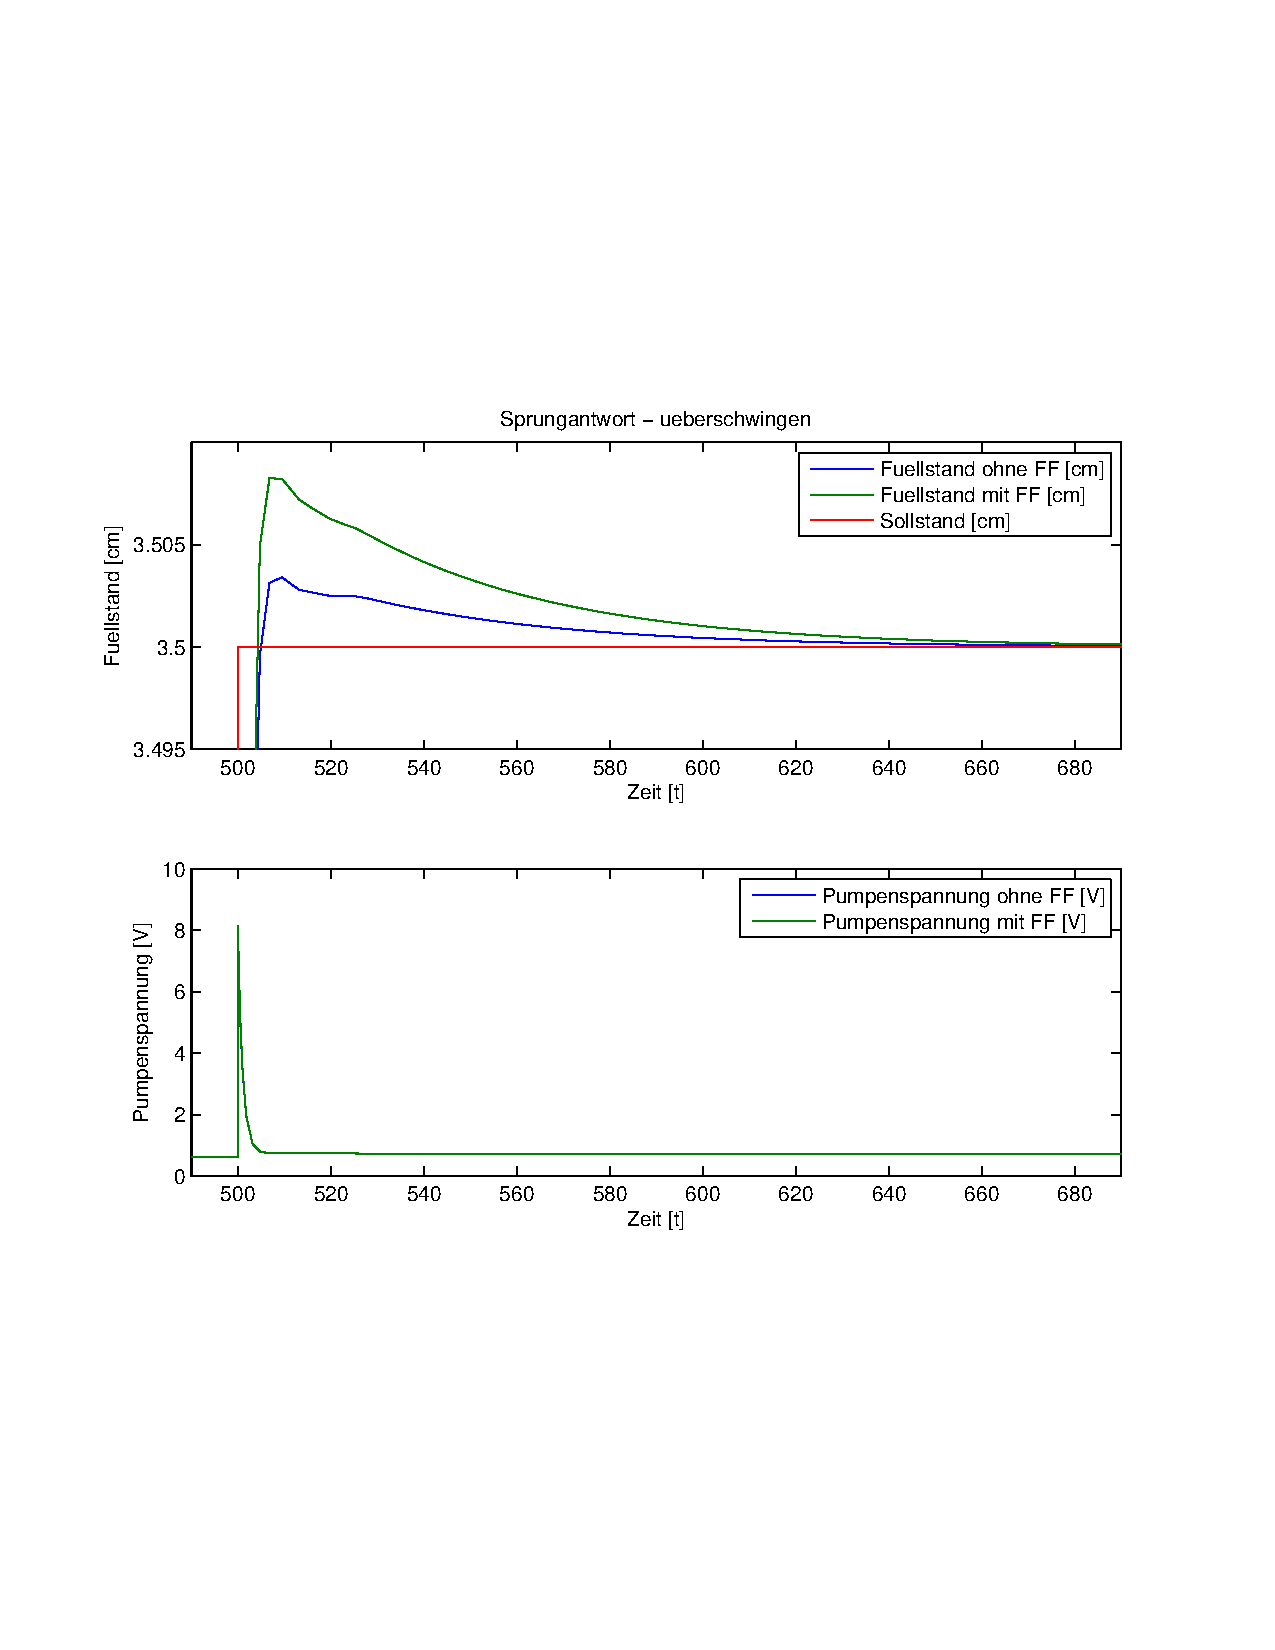
\includegraphics[width=1.\textwidth]{13/L5_step_overshoot_plot.pdf}
        \caption{Überschwingen im Arbeitsbereich von $G_5(s)$}
    \end{subfigure}
    \caption{Vergleich der Schrittantworten mit und ohne Vorsteuerung}
\end{figure}

\begin{figure}[h!]
    \begin{subfigure}{0.475\textwidth}
        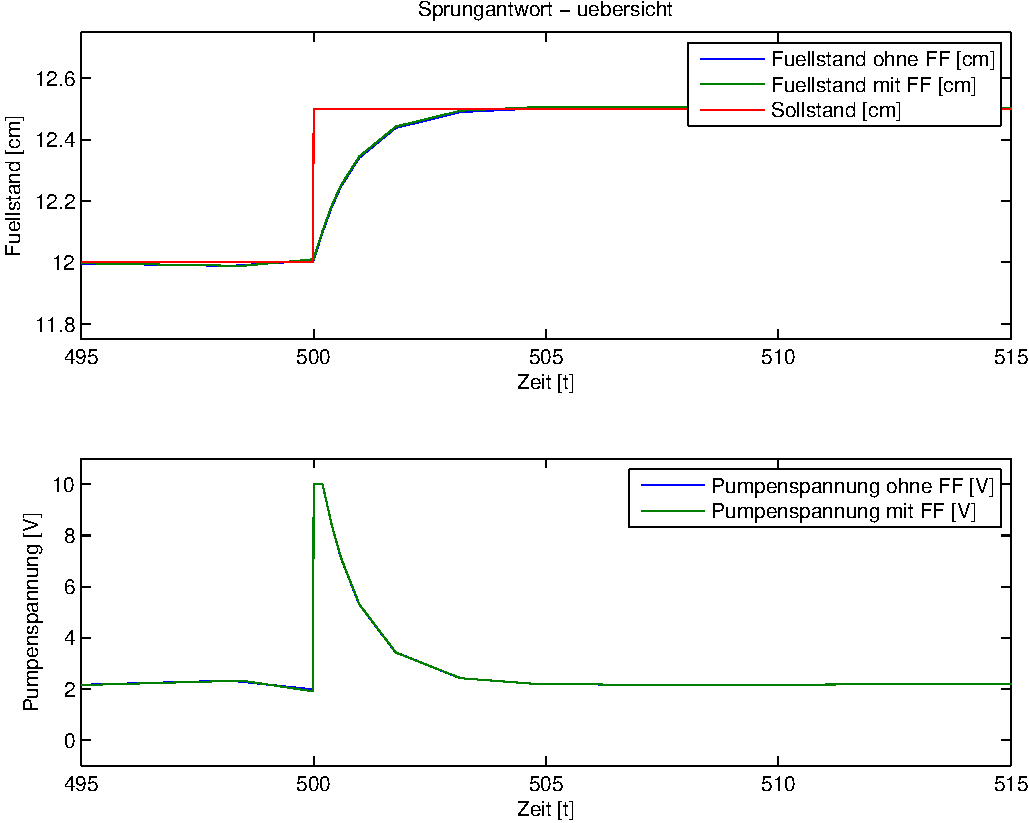
\includegraphics[width=1.\textwidth]{13/L7_step_overview_plot.pdf}
        \caption{Schrittantwort im Arbeitsbereich von $G_7(s)$}
    \end{subfigure}
    \hfill{}
    \begin{subfigure}{0.475\textwidth}
        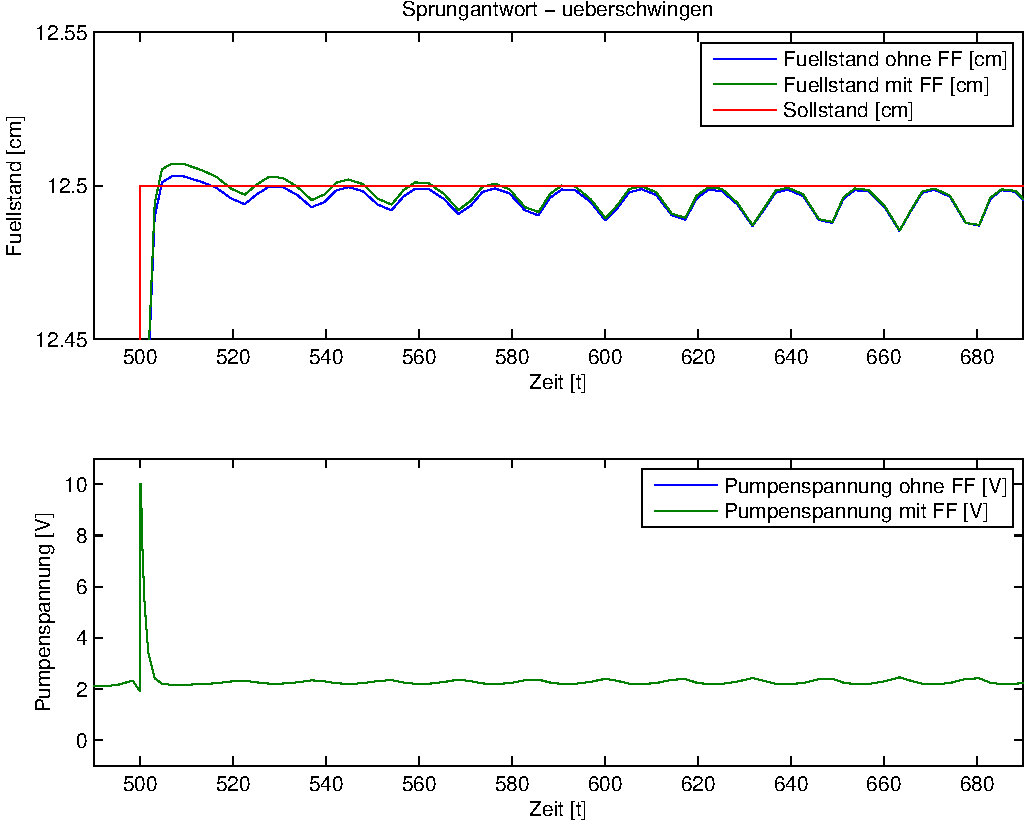
\includegraphics[width=1.\textwidth]{13/L7_step_overshoot_plot.pdf}
        \caption{Überschwingen im Arbeitsbereich von $G_7(s)$}
    \end{subfigure}
    \caption{Vergleich der Überschwinger mit und ohne Vorsteuerung}
\end{figure}

